\documentclass[dvipsnames]{beamer}

\usepackage{xcolor}
\usepackage{tikz}
\usepackage{xspace}
\usepackage{capt-of}
\usepackage{caption}
\usepackage{amsmath}
\usepackage{array}
\usepackage{tabularx}
\usepackage{booktabs}
\usepackage[export]{adjustbox}
\usepackage{graphicx}
\usepackage{eso-pic}  % For background image positioning
\usepackage{feynmp}
\usepackage{feynmp-auto}
\usepackage{listings}

\usepackage{hepparticles}
\usepackage{heppennames2}

\DeclareGraphicsRule{*}{mps}{*}{} 

\newcommand{\fb}{\ensuremath{\mathrm{fb}^{-1}}\xspace}

\setbeamertemplate{caption}[numbered]
\setlength\abovecaptionskip{0ex}
\setlength\belowcaptionskip{1.5ex}

% Adds the CMS logo to all frames with a frametitle
% Note: The this is very fragile and the \vskip had to be set to counter extra space inserted by the tikzpicture
% Only apply this background on title frame
\newcommand{\addtitlebackground}{
  \begin{tikzpicture}[remember picture, overlay]
    \node[anchor=center, inner sep=0pt] at (current page.center) 
      {\includegraphics[width=\paperwidth,height=\paperheight]{images/PresentationBackground.png}};
  \end{tikzpicture}
}

\usetheme{CambridgeUS}

% Title info
\title[LIV]
{LIV Status Update}
\author[Furong Yan]{\emph{Furong Yan}}
\institute[]{On Behalf of the LIV Group}
\date{\today}

\begin{document}

\section{Basics}
\subsection{LB Dataset}

\begin{frame}{Data Structure}

\begin{itemize}
  \item One row = one lumiblock (LB)
  \item 16 columns (order in file)
\end{itemize}

\vspace{0.4em}

\[
\small
\hspace{-0.5em}
\underbrace{
\begin{array}{l}
\texttt{FillNum},\ \texttt{RunNum},\ \texttt{LBNum},\\
\texttt{LBStart},\ \texttt{LBEnd},\ \texttt{LBLive},\ \texttt{LBFull}
\end{array}
}_{\textbf{Timing / LB skeleton}}
\quad\oplus\quad
\underbrace{
\begin{array}{l}
\texttt{OffMu},\ \texttt{PassGRL},\ \texttt{OffLumi},\\
\texttt{TightModLumi},\ \texttt{TightModLumiErr},\\
\texttt{ZeeEffComb},\ \texttt{ZeeErrComb},\\
\texttt{ZmumuEffComb},\ \texttt{ZmumuErrComb}
\end{array}
}_{\textbf{$N_Z$-related payload (rate / corrections)}}
\]

\vspace{0.5em}

\begin{itemize}
  \item Scramble: keep cols 1--7 fixed, shuffle rows of cols 8--16 as a block
  
  \item Why \texttt{PassGRL} is in the shuffled block?
    % \begin{itemize}
    %   \item selection mask? time-correlated veto structure?
    %   \item if already GRL-cleaned (mostly 1s), harmless; otherwise, shuffling changes window function
    % \end{itemize}
\end{itemize}

\end{frame}

\subsection{Analysis Setup}
\begin{frame}{Z counting}

Per-channel expected Z yield:
\vspace{-0.4em}
\[
N_Z^{ch}(\mathrm{LB}) \sim \mathrm{Poisson}\!\left(\lambda^{ch}(\mathrm{LB})\right)
\]
\vspace{-0.8em}
\[
\lambda^{ch}(\mathrm{LB})
=
\sigma_Z^{\rm fid}
\cdot A_{ch}
\cdot \epsilon_{ch}(\mathrm{LB})
\cdot F^{ch}_{\rm MC}\!\left(\mu(\mathrm{LB})\right)
\cdot \mathcal{L}(\mathrm{LB})
\]

\vspace{0.8em}

Correction factor:
\vspace{-0.4em}
\[
\texttt{ZcountCorr}^{ch}(\mathrm{LB}) = \epsilon_{ch}(\mathrm{LB})\cdot F^{ch}_{\rm MC}\!\left(\mu(\mathrm{LB})\right)
\]
\vspace{-1.2em}
\[
N_{Z,\mathrm{corr}}^{ch}(\mathrm{LB})=\frac{N_Z^{ch}(\mathrm{LB})}{\texttt{ZcountCorr}^{ch}(\mathrm{LB})}
\]

\vspace{0.8em}

Combine channels (optional): $N_{Z,\mathrm{corr}}^{\rm tot} = N_{Z,\mathrm{corr}}^{ee} + N_{Z,\mathrm{corr}}^{\mu\mu}$


\end{frame}


\begin{frame}{Phase}

\begin{itemize}
    \item Define a phase $\phi \in [0,1)$ for a chosen period \texttt{per}:
\end{itemize}

\vspace{-0.4em}
\[
t_{\rm mid}=\frac{t_{\rm start}+t_{\rm end}}{2},\qquad
\phi=\frac{\mathrm{mod}\!\left(\frac{t_{\rm mid}-t_{\rm shift}}{3600},\ \texttt{per}\right)}{\texttt{per}}
\in [0,1)
\]

\vspace{1.2em}

\begin{itemize}
  \item Phase binning: choose \texttt{nbin} bins in $\phi\in[0,1)$, assign each LB to a phase bin $k$
  \vspace{0.4em}
  \item For each bin $k$, accumulate corrected yield and luminosity:
\end{itemize}

\vspace{-0.2em}
\[
N_k=\sum_{\mathrm{LB}\in k} N_{Z,\mathrm{corr}}(\mathrm{LB}),\qquad
L_k=\sum_{\mathrm{LB}\in k} \mathcal{L}(\mathrm{LB})
\]

\end{frame}


\begin{frame}{Double Ratio}

\begin{itemize}
  \item ``Single ratio'' (rate-like quantity):
\end{itemize}

\vspace{-0.2em}
\[
R_{\rm single}(k)=\frac{N_k}{L_k}
\]

\vspace{0.3em}

\begin{itemize}
  \item Normalize both histograms to remove global scale:
\end{itemize}

\vspace{-0.2em}
\[
\tilde N_k=\frac{N_k}{\sum_j N_j},\qquad
\tilde L_k=\frac{L_k}{\sum_j L_j}
\]

\vspace{0.3em}

\begin{itemize}
  \item Double ratio (ratio-of-ratios):
\end{itemize}

\vspace{-0.2em}
\[
R_D(k)=\frac{\tilde N_k}{\tilde L_k}
=\frac{N_k/L_k}{\left(\sum_j N_j\right)/\left(\sum_j L_j\right)}
\]

\end{frame}

\begin{frame}{Intepretation}

\begin{itemize}
  \item SME term enters fiducial cross section:
\end{itemize}

\vspace{-0.8em}
\[
\sigma(t)=\sigma_0\,[1+a\,f(\phi(t))]
\]

\vspace{0.4em}

\begin{itemize}
  \item corrected yield
\end{itemize}

\vspace{-1.2em}
\[
\mathbb{E}[N_{Z,\mathrm{corr}}^{\ell}]=\mathbb{E}\!\left[\frac{N_\ell}{\epsilon_\ell F_{\rm MC}(\mu_\ell)}\right]=A\,\sigma(t_\ell)\,\mathcal{L}_\ell
\]

\vspace{0.4em}

\begin{itemize}
  \item double ratio
\end{itemize}

\vspace{-1.2em}
\[
\mathbb{E}[R_D(k)]
=\frac{\mathbb{E}[N_k/L_k]}{\mathbb{E}[(\sum_j N_j)/(\sum_j L_j)]}
=\frac{1+a\,f(\phi_k)}{1+a\,\langle f\rangle_L}
\]

\vspace{0.4em}

\begin{itemize}
  \item Condition for $\mathbb{E}[R_D(k)]=1+a\,f(\phi_k)$:
  \vspace{0.4em}
  \begin{itemize}
    \item $\langle f\rangle_L=0$ (mean over LBs vanishes; uniform phase coverage)
  \end{itemize}
\end{itemize}

\end{frame}

\subsection{Toy Model}
\begin{frame}{DB Plot -- 2015+2016}

\centering
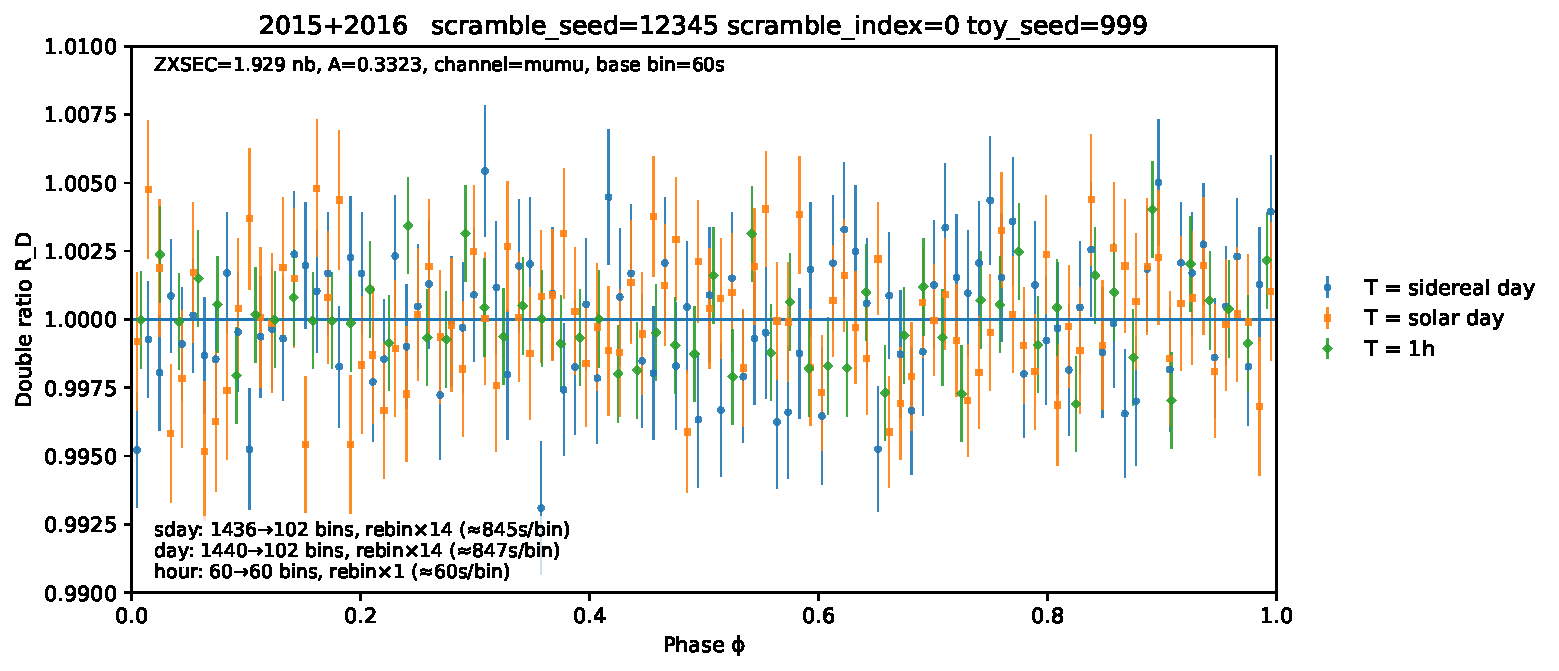
\includegraphics[width=\linewidth]{plots/xs(sigmaFID)_phase(60sec)_2015+2016.pdf}

\end{frame}

\begin{frame}{DB Plot -- 2017}

\centering
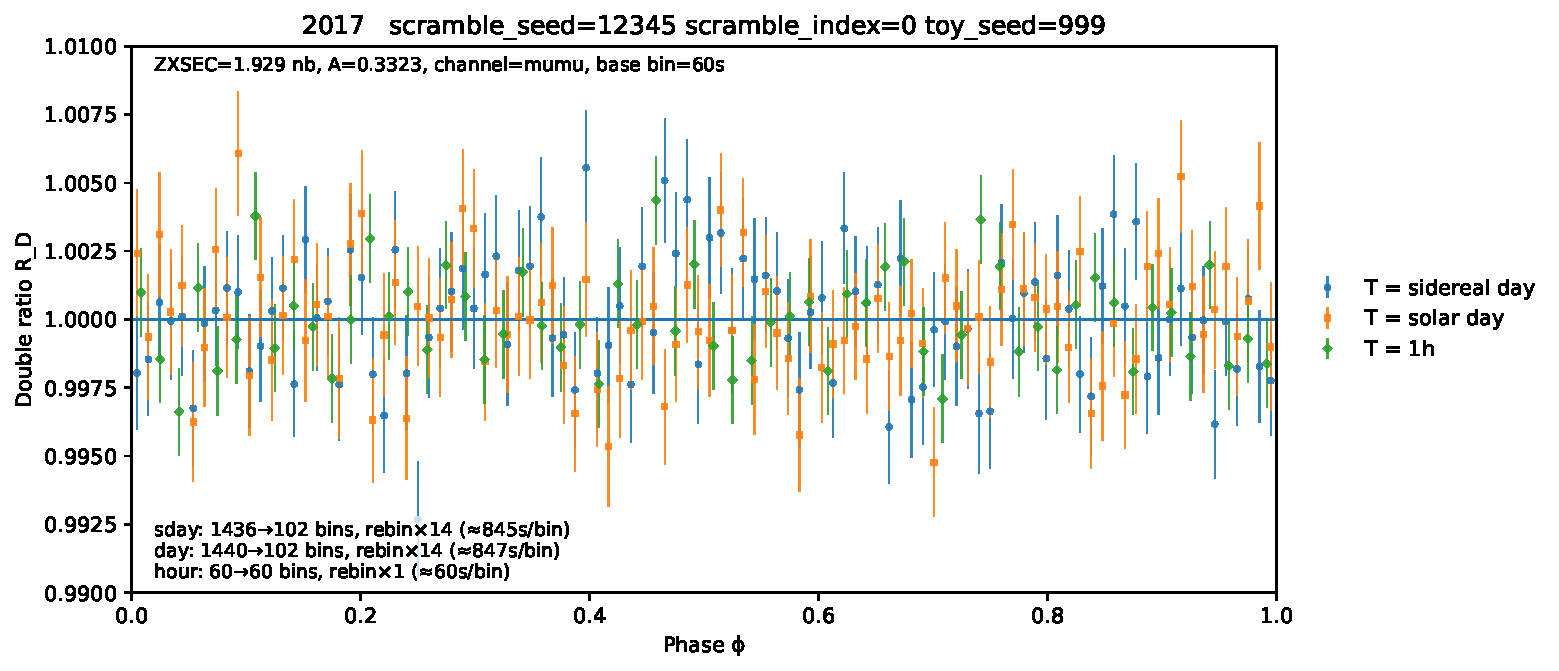
\includegraphics[width=\linewidth]{plots/xs(sigmaFID)_phase(60sec)_2017.pdf}

\end{frame}

\begin{frame}{DB Plot -- 2018}

\centering
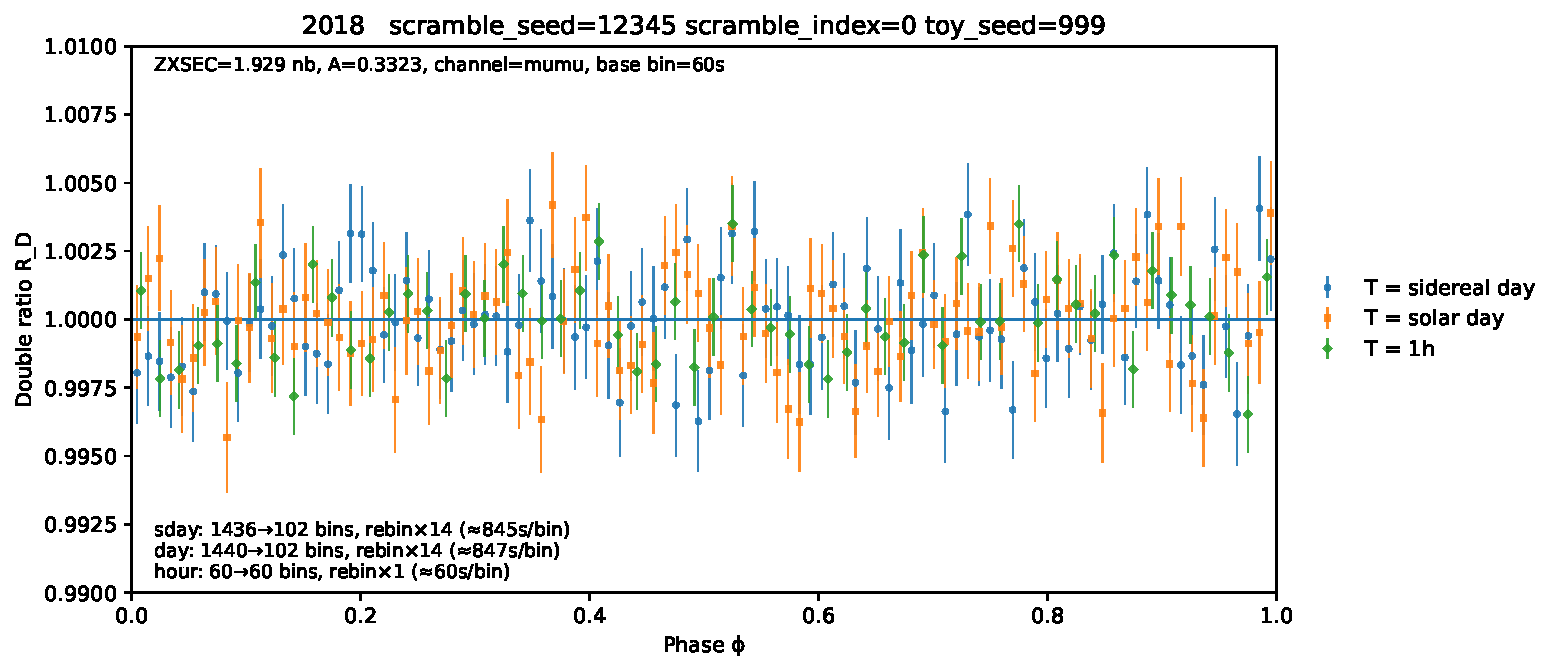
\includegraphics[width=\linewidth]{plots/xs(sigmaFID)_phase(60sec)_2018.pdf}

\end{frame}

\section{Blind Analysis Framework}
\subsection{Data Scrambling}

\begin{frame}{Scrambling Strategy}
    \begin{itemize}
        \item \textbf{Objective}: Destroy physics correlations (sidereal time vs data) while preserving temporal coverage.
        \vspace{0.6em}
        \item \textbf{Method}: Block Shuffle of the dataset across four years.
        \begin{itemize}
            \item \textbf{Fixed Columns}:
            \begin{itemize}
                \item \texttt{RunNum, LBNum, LBStart, LBEnd, LBLive}
            \end{itemize}
            \vspace{0.3em}
            \item \textbf{Shuffled Columns}:
            \begin{itemize}
                \item \texttt{ZllLumi, OffLumi}
            \end{itemize}
        \end{itemize}
        \vspace{0.6em}
        \item \textbf{Quantity}: 1000 scrambles, randomized by a deterministic pattern.
    \end{itemize}
\end{frame}

\begin{frame}{Demo - DR plot of Scrambled Dataset}

\hspace*{-1.1em}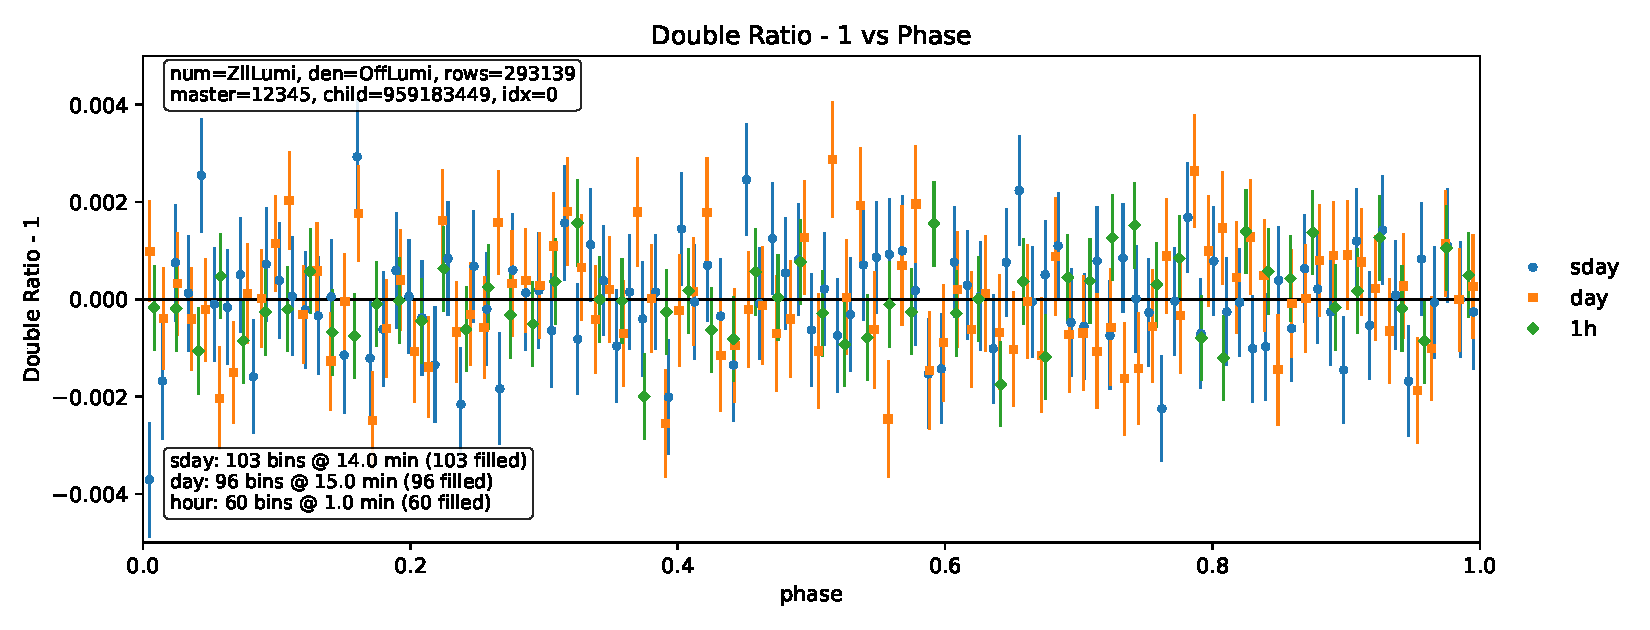
\includegraphics[width=1.08\linewidth]{plots/scramble_0_double_ratio.pdf}

\end{frame}

\section{Validation Results}

\begin{frame}{Signal Injection Test}
% \vspace{-0.2em}
\begin{itemize}
    \item \textbf{Method}: Injection of $c_{u,YZ} = 10^{-4}$ into 10 scrambles vs 10 independent null scrambles.
    \item \textbf{Observation}: A coherent modulation is visible above the noise floor.
\end{itemize}
    
\vspace{-0.1em}
\centering
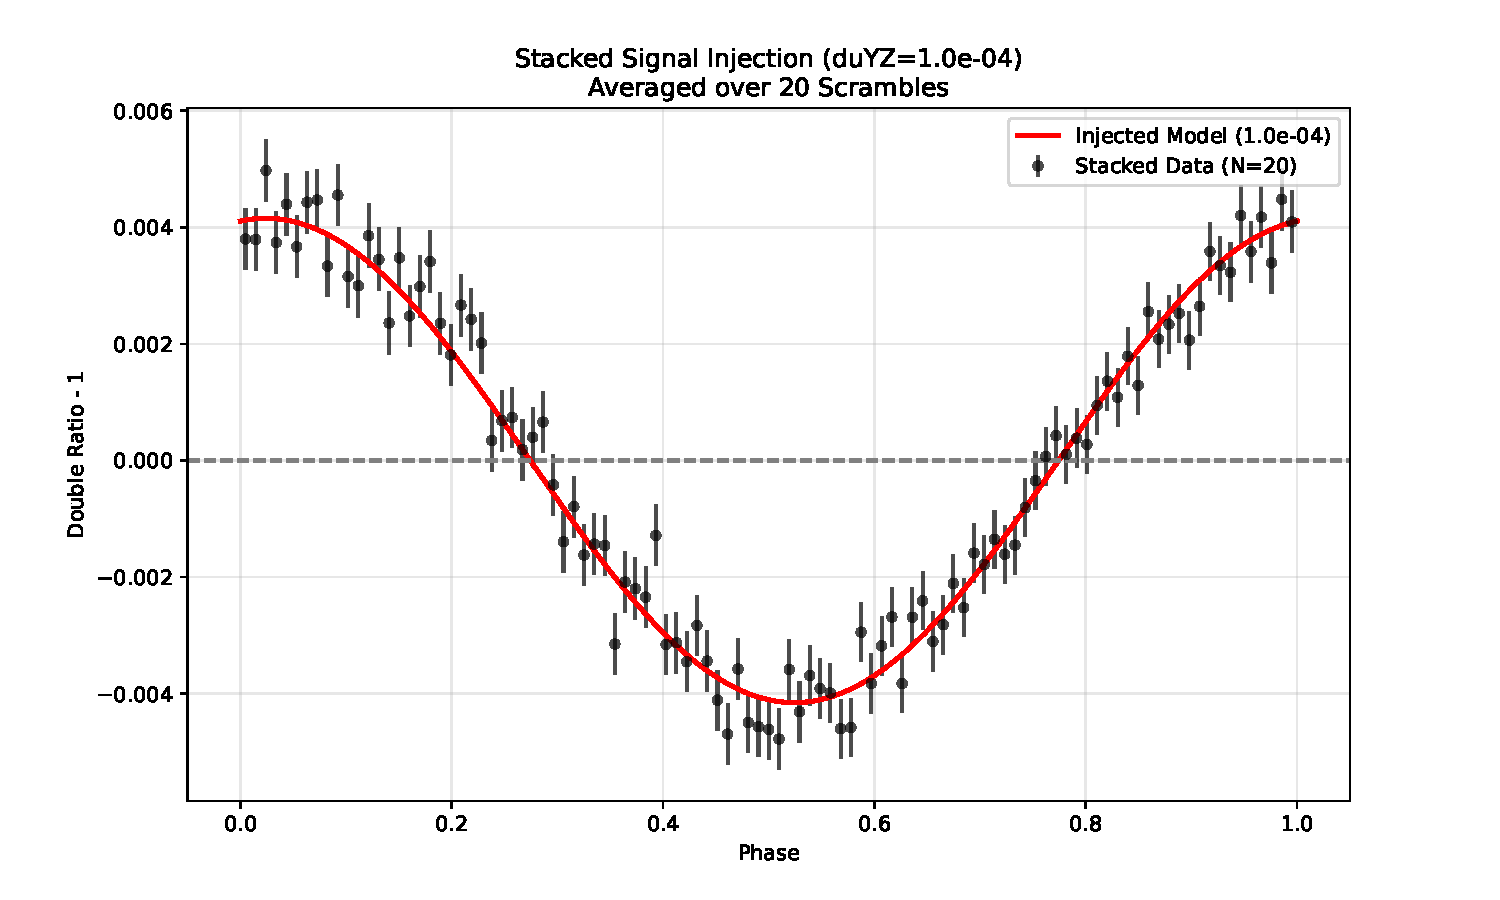
\includegraphics[width=0.85\linewidth]{plots/injection_stacked_duYZ_1e-4.pdf}
\end{frame}

\begin{frame}{Low-Signal Injection Test}
% \vspace{-0.2em}
\begin{itemize}
    \item Now change the signal strength to $c_{u,YZ} = 10^{-5}$. Expect it to be buried by the $\sqrt{N}$ statistical noise of the sample.
\end{itemize}
    
\vspace{-0.1em}
\centering
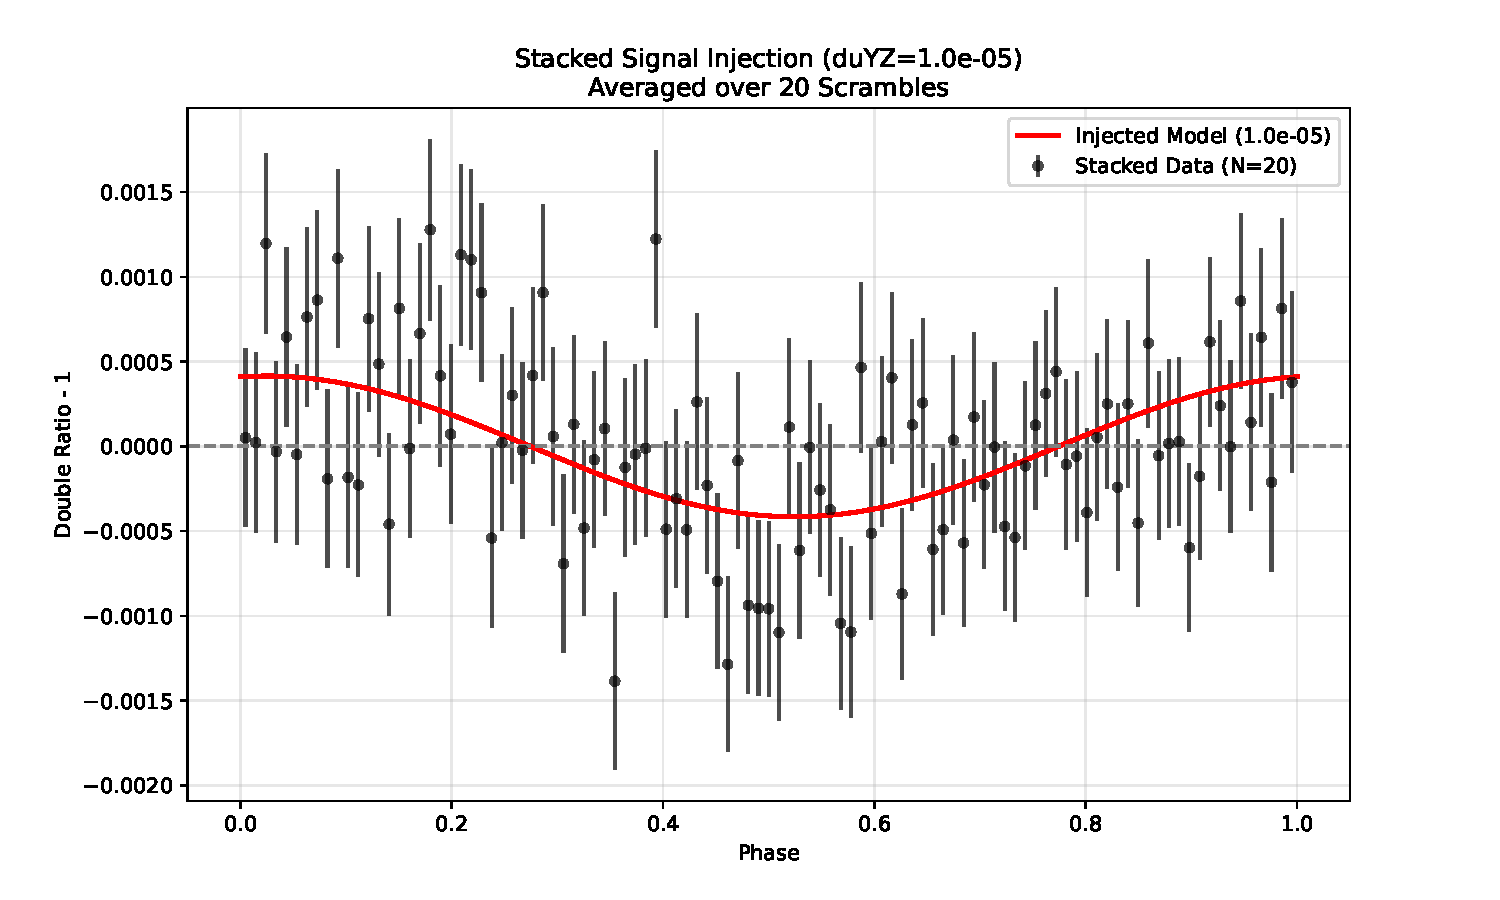
\includegraphics[width=0.85\linewidth]{plots/injection_stacked_duYZ_1e-5.pdf}
\end{frame}

\begin{frame}{Systematics Control}
    \begin{itemize}
    \setlength\itemsep{0.6em}
        \item \textbf{Detector Acceptance}: Raw luminosity ratios show $\mathcal{O}(10^{-3})$ variations.
        \item \textbf{Null Hypothesis Test}: If the Double Ratio fails to cancel these acceptance effects, we would expect residual structure in the null scrambles.
        \vspace{0.3em}
        \item \textbf{Observation}: 
        \begin{itemize}
        \setlength\itemsep{0.3em}
            \item Null scrambles are consistent with flat noise within $< 10^{-4}$.
            \item Degeneracy of the operators: XZ, YZ, XXYY and XY.
        \end{itemize}
    \end{itemize}
\end{frame}

\section{Statistical Profile}
\begin{frame}{Null Hypothesis Tests (1000 Scrambles)}
    \centering
    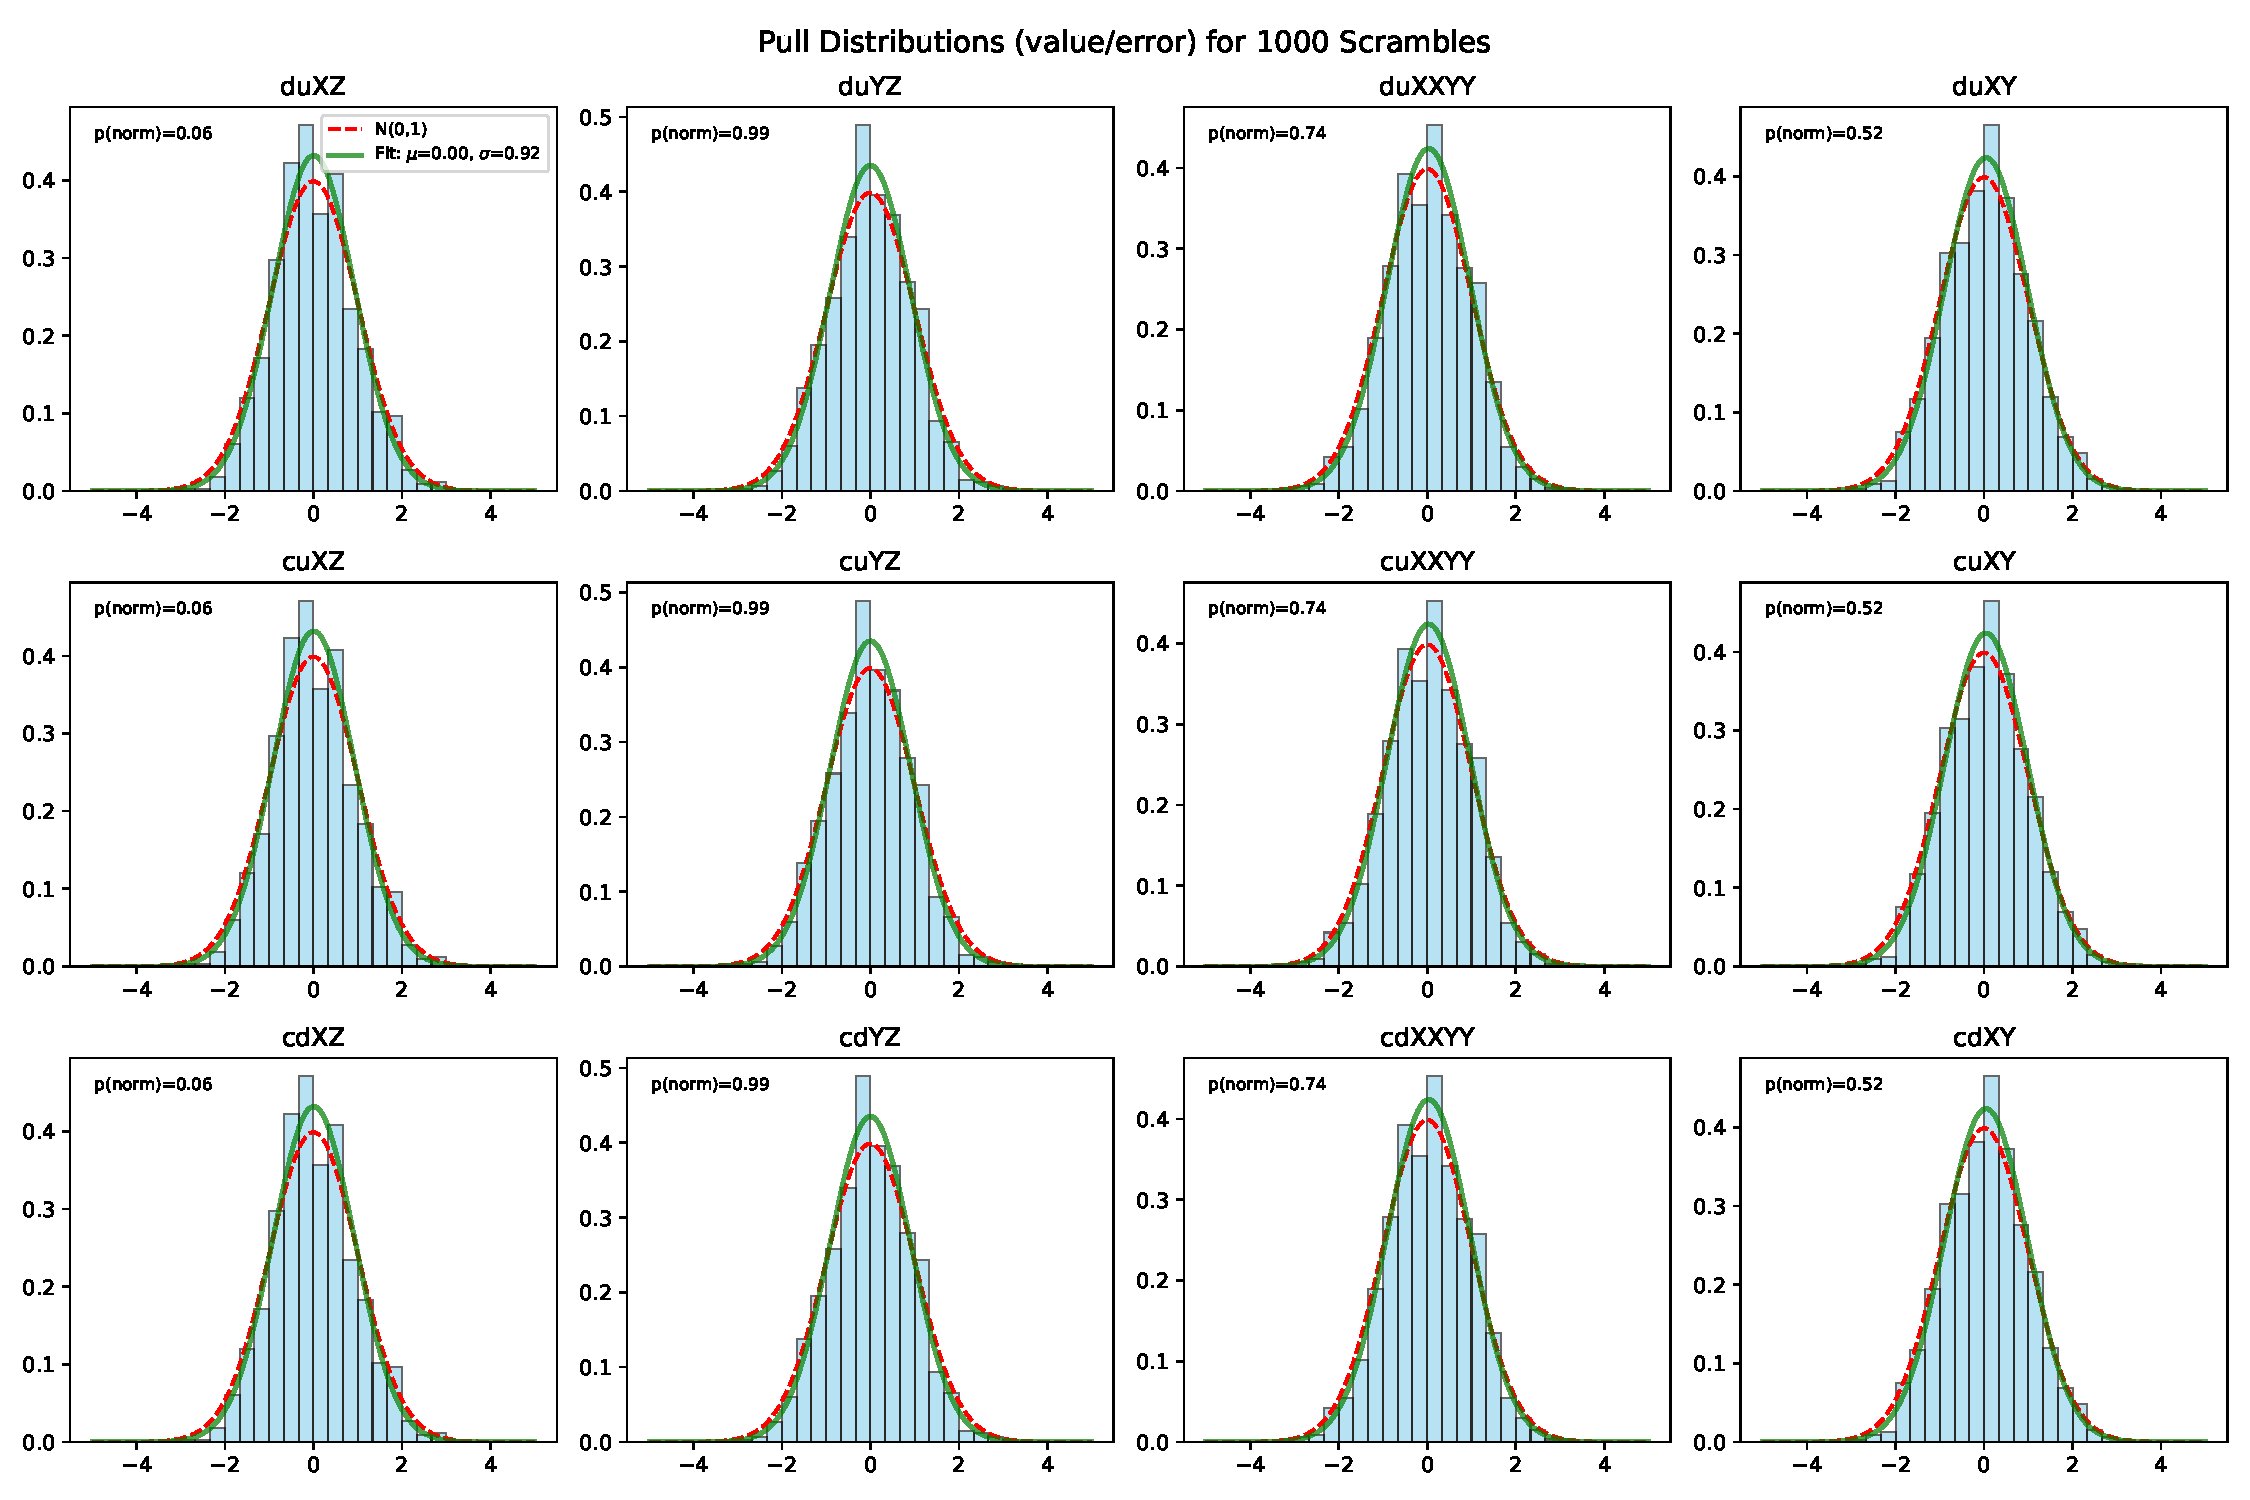
\includegraphics[width=0.88\linewidth]{plots/pull_distributions.pdf}
    \captionof{figure}{Pull distributions $(c_{fit})/\sigma_{fit}$ for 1000 null scrambles.}
\end{frame}

\appendix
\section{Backup}

\begin{frame}[fragile]{Technical Implementation of Scrambling}

\textbf{RNG Architecture}:
\vspace{0.6em}
    \begin{itemize}
    \setlength\itemsep{0.3em}
        \item \textbf{Master Seed}: A single integer (e.g., \texttt{12345}) defines the campaign.
        \item \textbf{Child Seeds}: uncorrelated states generated by master seed.
    \end{itemize}
    
    \vspace{0.5em}
    
\begin{lstlisting}[language=Python]
ss_master = np.random.SeedSequence(masterseed)
ss_samples = ss_master.spawn(n)
for i, ss in enumerate(ss_samples):
    rng = np.random.default_rng(ss) 
    yield i, scramble_one(base, rng)
\end{lstlisting}

\end{frame}

\end{document}
